%\section{Models and parameter estimation (NH)}
%\input Sections/model_Nancy.tex

We first remind the reader of the definition of a hidden Markov model and extend this to the CarHMM. We then introduce hierarchical structures within HMMs using both the short-time Fourier transform (STFT) and the hierarchical hidden Markov model (HHMM)

%%%%%%%%%%%%%%%%%%%%%%%%%%%%%%%%%%%%%%%%%
\subsection{The hidden Markov model (HMM)}

A \textit{hidden Markov model}  is comprised of a sequence of  unobserved states $X_t$, $t = 1, \ldots, T$, and an associated sequence of  possibly high-dimensional observations $Y_t$, $t = 1, \ldots, T$,
The $Y_t$s are often referred to as ``emissions'' and the index $t$ typically refers to time. 
The $X_t$s form a Markov chain and take possible values $1, \ldots, N$. Their distribution is governed by the distribution of the initial state $X_1$ and the $N \times N$ transition probability matrix $\Gamma$ where $\Gamma_{ij} = \Pr(X_{t+1} = j | X_t = i)$, for $t=1,\ldots, T-1$, and $i, j = 1,\ldots, N$. 
%
We assume that $X_1$ follows the chain's stationary distribution, which is denoted by $\delta \in \bbR^N$, with $i$th component
$\delta_i = \Pr\{X_1 = i\},~ i = 1,\ldots,N.$
%
Recall that a Markov chain's stationary distribution is determined by its probability transition matrix via $\delta = \delta \Gamma$ and $\sum_{i=1}^N \delta_i = 1$.
%
The distribution of an emission $Y_t$ depends only on the corresponding state $X_t$ and no other observations or hidden states: $p\left(y_t|\{X_1,\ldots, X_T\},\{Y_1,\ldots, Y_T\}/ \{Y_t\}\right) = p(y_t|X_t)$.
%
These conditional distributions are governed by state-dependent parameters: if $X_t = i$, the state-dependent parameter is $\theta^{(i)}$ and we denote the conditional distribution of $Y_t$ given $X_t=i$ by its conditional density or probability mass function, denoted $f^{(i)}(\cdot ; \theta^{(i)})$, or sometimes  $f^{(i)}(\cdot)$.
%
(Fig \ref{fig:HMM}) represents the dependence structure.

To find the maximum likelihood estimates of the parameters $\Gamma$ and $\Theta \equiv (\theta^{(1)},\ldots,\theta^{(N)})$, let $y = (y_1,\ldots,y_T)$ be the observed emissions. 
 To facilitate calculations we write the likelihood $\calL_{\text{HMM}}$ in a specific form, using the  well-known \textit{forward algorithm} \citep{Zucchini:2016} as follows:
%
$$\calL_{\text{HMM}}(y;\Theta,\Gamma) = \delta P(y_1;\Theta) \prod_{t=2}^T \Gamma P(y_t;\Theta) \mathbf{1}_N$$
%
where $\mathbf{1}_N$ is an $N$-dimensional column vector of ones and
%
$P(y_t;\Theta)$ is an $N \times N$ diagonal matrix with $ii$th entry  $f^{(i)}(y_t; \theta^{(i)})$.
%

We will always parameterize transition probability matrices to remove the constraints that the entries of the matrix are non-negative and that the rows sum to 1.  We do this by parameterizing the $N \times N$ transition probability matrix $\Gamma$ using $\eta \in \bbR^{N \times N}$ \citep{Barajas:2017}:
%
\[
\Gamma_{ij} = \frac{\exp(\eta_{ij})}{\sum_{k=1}^N \exp(\eta_{ik})}, 
\]
%
setting $\eta_{ii}$  to zero, $i=1,\ldots, N$, for identifiability.  Then $\calL_{\text{HMM}}(y;\Theta,\Gamma)$ can be maximized using any numerical optimizer.  For simplicity, we will continue to use $\Gamma$ in our notation, suppressing the reparameterization in terms of  $\eta$.

\begin{figure}[ht]
	\centering
	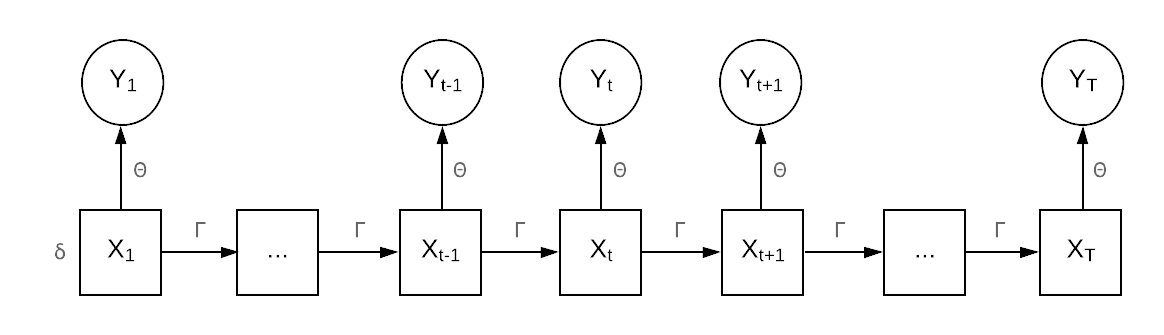
\includegraphics[width=5in]{../Plots/HMM.png}
	\caption{Graphical representation of a traditional HMM.}
	\label{fig:HMM}
\end{figure}


%%%%%%%%%%%%%%%%%%%%%%%%%%%%%%%%%%%%%%%%%
\subsection{The conditionally auto-regressive hidden Markov model (CarHMM)}

One of the key assumptions of an HMM is \textit{conditional independence} between observations, given the state sequence.  Therefore, traditional HMMs do not hold when the observations exhibit certain forms of significant correlation in time.

One way to model extra correlation in an HMM type structure is via a CarHMM, or \textit{conditionally auto-regressive hidden Markov model}, introduced by \citep{Lawler:2019}. Like a traditional HMM, A CarHMM is made up of a Markov chain of unobserved states $X_1,\ldots, X_T$ that can take on values $1, \ldots, N$, with transition probability matrix $\Gamma$ and initial distribution $\delta$ equal to the stationary distribution. Unlike a traditional HMM, the CarHMM assumes that the distribution of the $t$th emission, $Y_t$, conditional on $X_1,\ldots, X_T$ and $ \{Y_1,\ldots, Y_{t-1}\}$, depends on both $X_t$ \textit{and} $Y_{t-1}$. 
The first emission $Y_1$ is assumed to be fixed as an initial value which does not depend upon $X_1$. (Fig \ref{fig:CarHMM}) shows the structure of a CarHMM.

\begin{figure}[ht]
	\centering
	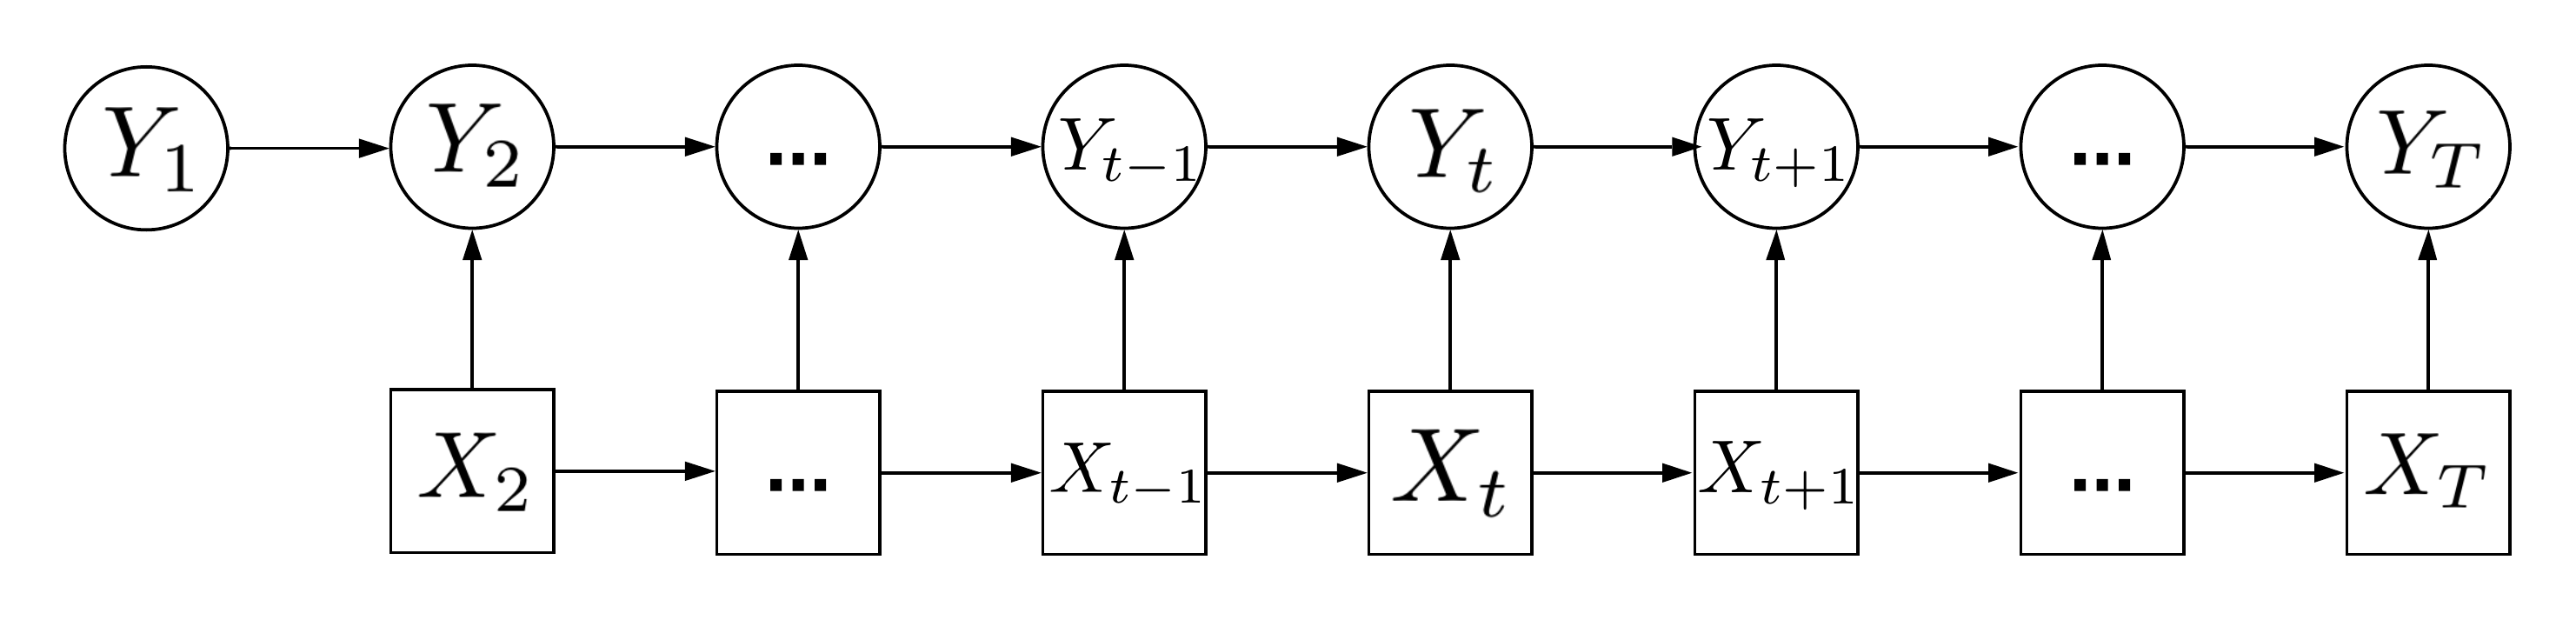
\includegraphics[width=5in]{../Plots/CarHMM.png}
	\caption{Graphical representation of a traditional CarHMM.}
	\label{fig:CarHMM}
\end{figure}

%
We denote the conditional distribution of $Y_t$ given $Y_{t-1}= y_{t-1}$ and $ X_t=i$ as $f^{(i)}( \cdot | y_{t-1})$ or as
$f^{(i)}( \cdot | y_{t-1}; \theta^{(i)})$.
As an example, we could assume that this conditional distribution is normal with parameters $\theta^{(i)} = \{\mu^{(i)},\sigma^{2(i)},\phi^{(i)}\}$, with:
%
\[
\mathbb{E}(Y_t|Y_{t-1} = y_{t-1},X_t=i) = \phi^{(i)} ~ y_{t-1} ~+ ~(1-\phi^{(i)})  ~\mu^{(i)}
\]
and
\[
\mathbb{V}(Y_t| Y_{t-1} =y_{t-1}, X_t = i) = \sigma^{2(i)}.
\]
%
{\bf{Ah - now I see the issue about changing states.  It would be great to have something about the distribution of $Y_t$ given $X_t=i, X_{t-1}=j$. You'd want a different conditional distribution, depending on if $i=j$ or not.
}}
%
The CarHMM therefore explicitly models auto-correlation into the emission distributions of the HMM while maintaining the structure needed to write the likelihood using the forward algorithm. In our normal model formulation, we have added only one additional parameter, $\phi^{(i)}$,  per possible hidden state. 

The likelihood for the CarHMM can be easily calculated using the forward algorithm.  As previously, let $y$ be the vector of observed emissions.  Then
\begin{equation}
\calL_{\text{CarHMM}}(y;\Theta,\Gamma) = \delta \prod_{t=2}^T \Gamma P(y_t;\Theta) \mathbf{1}_N
\label{CarHMM_likelihood}
\end{equation}
where
%
$P(y_t;\Theta)$ is an $N \times N$ diagonal matrix with $ii$th entry equal to $f^{(i)}(y_t|y_{t-1}; \theta^{(i)})$.
%

%%%%%%%%%%%%%%%%%%%%%%%%%%%%%%%%%%%%%%%%%
\subsection{The hierarchical hidden Markov model (HHMM)}

A hierarchical hidden Markov model contains two process levels, a coarse-scale process and a fine-scale process.  The coarse-scale process is a hidden Markov model as defined in the previous subsection,  with  $X_1\ldots, X_T$ the unobserved Markov chain of states and $Y_1,\ldots, Y_T$ the corresponding observed responses.  The possible states are $1,\ldots, N$.   
%

For each value of $t$, the state $X_t$ emits not only $Y_t$ but also  a sequence of unobserved states, 
$X_t^* \equiv (X_{t,1}^*,\ldots, X_{t,T_t^*})$ and a sequence of observed emissions, 
$Y_t^* \equiv (Y_{t,1}^*,\ldots, Y_{t,T_t^*})$. 
These form our fine-scale process.
Conditional on the coarse-scale hidden state $X_t$, the joint fine-scale process,  $X_t^*$, $Y_t^*$, is a hidden Markov model with parameters depending on the value of $X_t$.  Specifically, given that $X_t=i$,   $X_t^*$ is a Markov chain with states $1,\ldots, N_t^*$ with 
%
\hfill\break{\bf{NH:  Do we write $1^*$? That's strange.}}
\hfill\break
%
 distribution of $X_t^*$, conditional on $X_t=i$,  given by an $N^*_t \times N^*_t$ transition probability matrix $\Gamma^{*(i)}$ and initial probability, denoted by the $N_t^*$-vector $\delta^{*(i)}$, which we take equal to the stationary distribution of the chain.     For simplicity, we  take $N_t^* \equiv N^*$ although this is not necessary.
%
The distribution of $Y_{t, t^*}$
given $X_{t, t^*}=i^*$ and $X_t=i$ is governed by a parameter  $\theta^{(i,i^*)}$, and has density or probability mass function denoted $f^{*(i,i^*)}\left(\cdot; \theta^{(i,i^*)}\right)$ or sometimes simply denoted by $f^{*(i,i^*)}(\cdot)$.
Let $\Theta^{*(i)}=\left(\theta^{(i,1)}, \ldots, \theta^{(i,N^*)}\right)$, the fine-scale emission parameter vector corresponding to $X_t=i$.
%
\hfill\break
{\bf{NH:  will there be some parameters that are common across the fine-scale emission distributions? Do we want to separate them out?\\
Also - I used left ( and right ) above to make the parentheses a little bigger.  I think it looks better.  So we may want to do this throughout.
$f^{*(i,i^*)}\left(\cdot; \theta^{(i,i^*)}\right)$ versus
$f^{*(i,i^*)}(\cdot; \theta^{(i,i^*)})$.
}}
\hfill\break
%
The dependencies among the processes are defined as follows.
%
Given the coarse-scale states, $X_1,\ldots, X_T$, and the coarse scale emissions,  
$Y_1,\ldots, Y_T$, the $T$ fine-scale processes $(X_1^*, Y_1^*), \ldots, (X_T^*, Y_T^*)$, are independent HMMs.  
%%
\hfill\break
{\bf{I think that works for the dependencies - might need to add more. Does that look OK to you?}}
%%

Due to the nested structure of the hierarchical hidden Markov model, the likelihood  is easy to calculate via the forward algorithm, just as for HMMs.
%
Let $y$ be the $T$-vector of the observed coarse-scale emissions and
$y^*$ be the $(T_1^* + \cdots T_T^*)$-vector of the observed fine-scale emissions.
%
Let $\Theta^*$ denote the collection of all fine-scale emission parameters,
$\Theta^{*(i)}$, $i=1,\ldots, N$, and let $\Gamma^*$ denote the collection of all fine-scale transition probability matrices, $\Gamma^{*(i)}$, $i=1,\ldots, N$.
%
Then the likelihood of the observed data is:
%
\[
\calL_{\text{HHMM}}(y,y^*;\Theta,\Theta^*,\Gamma,\Gamma^*) = \delta P(y_1,y_1^*;\Theta,\Theta^*,\Gamma^*) \prod_{t=2}^T \Gamma P(y_t,y_t^*;\Theta,\Theta^*,\Gamma^*) \mathbf{1}_N
\]
%
where 	$P(y_t,y_t^*;\Theta,\Theta^*,\Gamma^*)$ is an $N^ \times N$ diagonal matrix with $ii$th entry corresponding to $X_t=i$ and equal to 
$f^{(i)}(y_t)\calL_{\text{HMM}}\left(y_t^*;\Theta^{*(i)},
\Gamma^{*(i)}\right)$. 

For more information on specific considerations for HHMMs such as incorporating covariates into the probability transition matrix, model selection and model checking, see Adam et al \citep{Adam:2019}.

\begin{figure}[ht]
	\centering
	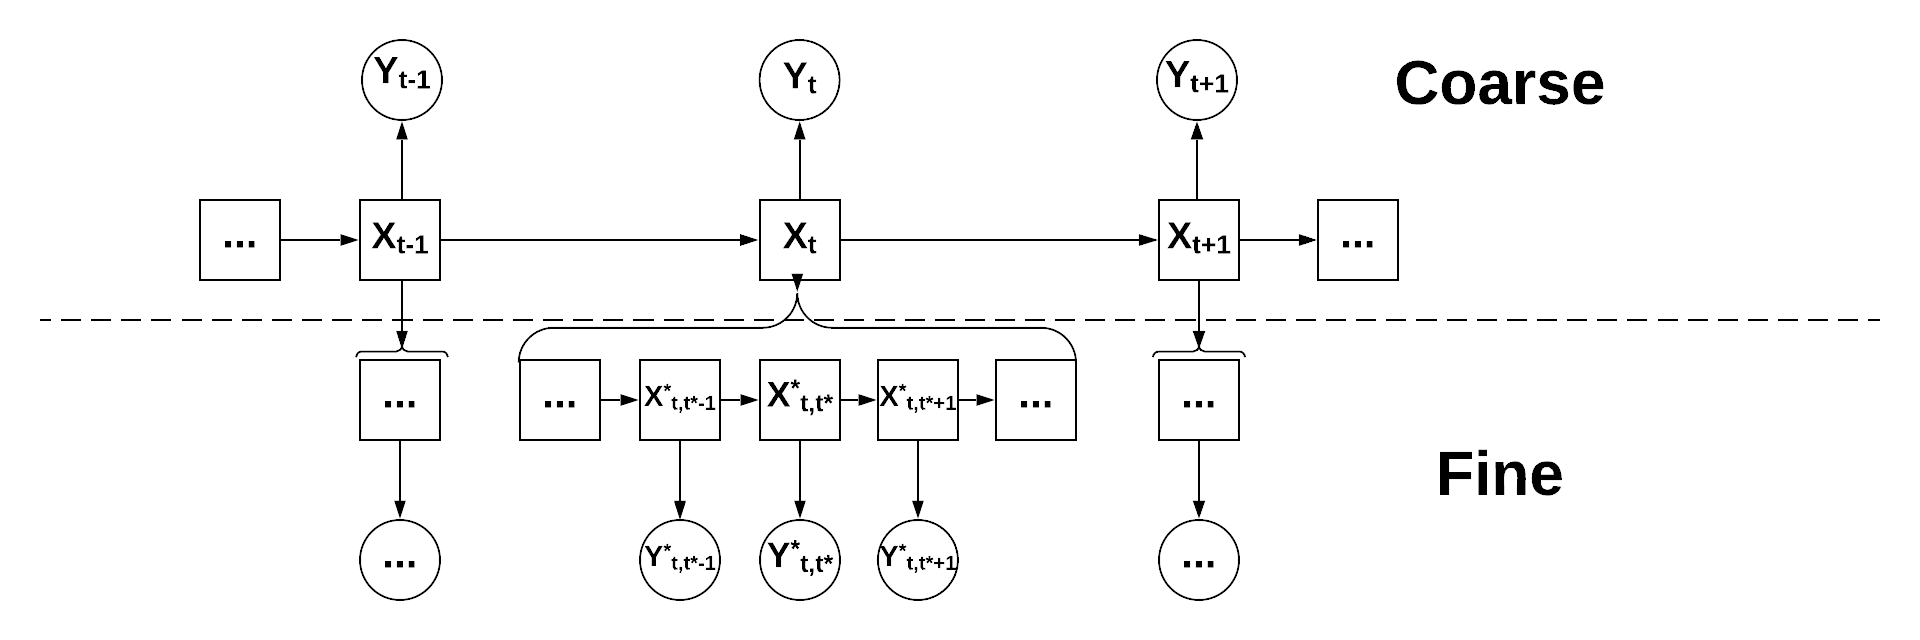
\includegraphics[width=5in]{../Plots/HHMM.png}
	\caption{Graphical representation of a traditional HHMM.}
	\label{fig:HHMM}
\end{figure}

% do I need this subsections
\subsection{Decoding}

{\bf{I'm stopping here.  Perhaps you can take a stab at revisions here?}}

